\chapter{Evaluation} \label{cha:evaluation}

% The outcome of the migration process is evaluated in the fifth chapter. The potential benefits and drawbacks of the serverless platform outlined in chapter 2 are used to reflect on the final artifact. The chapter includes approximations on measurable attributes such as hosting costs and performance as well as discussion on the more subjective attributes like maintainability and testability. The overall ease of development -- or developer experience -- is also addressed since it is one of the commonly reported pain points of serverless computing

% Finally in chapter \ref{cha:evaluation} the migration outcome is evaluated against the pre-migration application in terms of quality and ease of development.
Evaluation the outcome of migration process. Estimate the effects on performance and hosting costs. Weigh in on maintainability, testability, developer experience etc.

qualitative vs quantitative

% check example at https://onlinelibrary.wiley.com/doi/epdf/10.1002/spe.2608
How did the migration help in future extendability and maintenance of Image Manager?
- development perspective
  - less bundling/coupling
- operational perspective
  - ease of deployment
  - monitoring
- financial perspective
- performance perspective
  - cold start averted by 1) optionally using function warmer, 2) only having one synchronous bottleneck, otherwise event-driven
- others?

Old implementation's shortcomings of availability, scalability, cost-efficiency and isolation -- we're these addressed?

% got more or less cloud-ready? \parencite{pozdniakova17cloudready}

\begin{figure}[h]
  \centering
  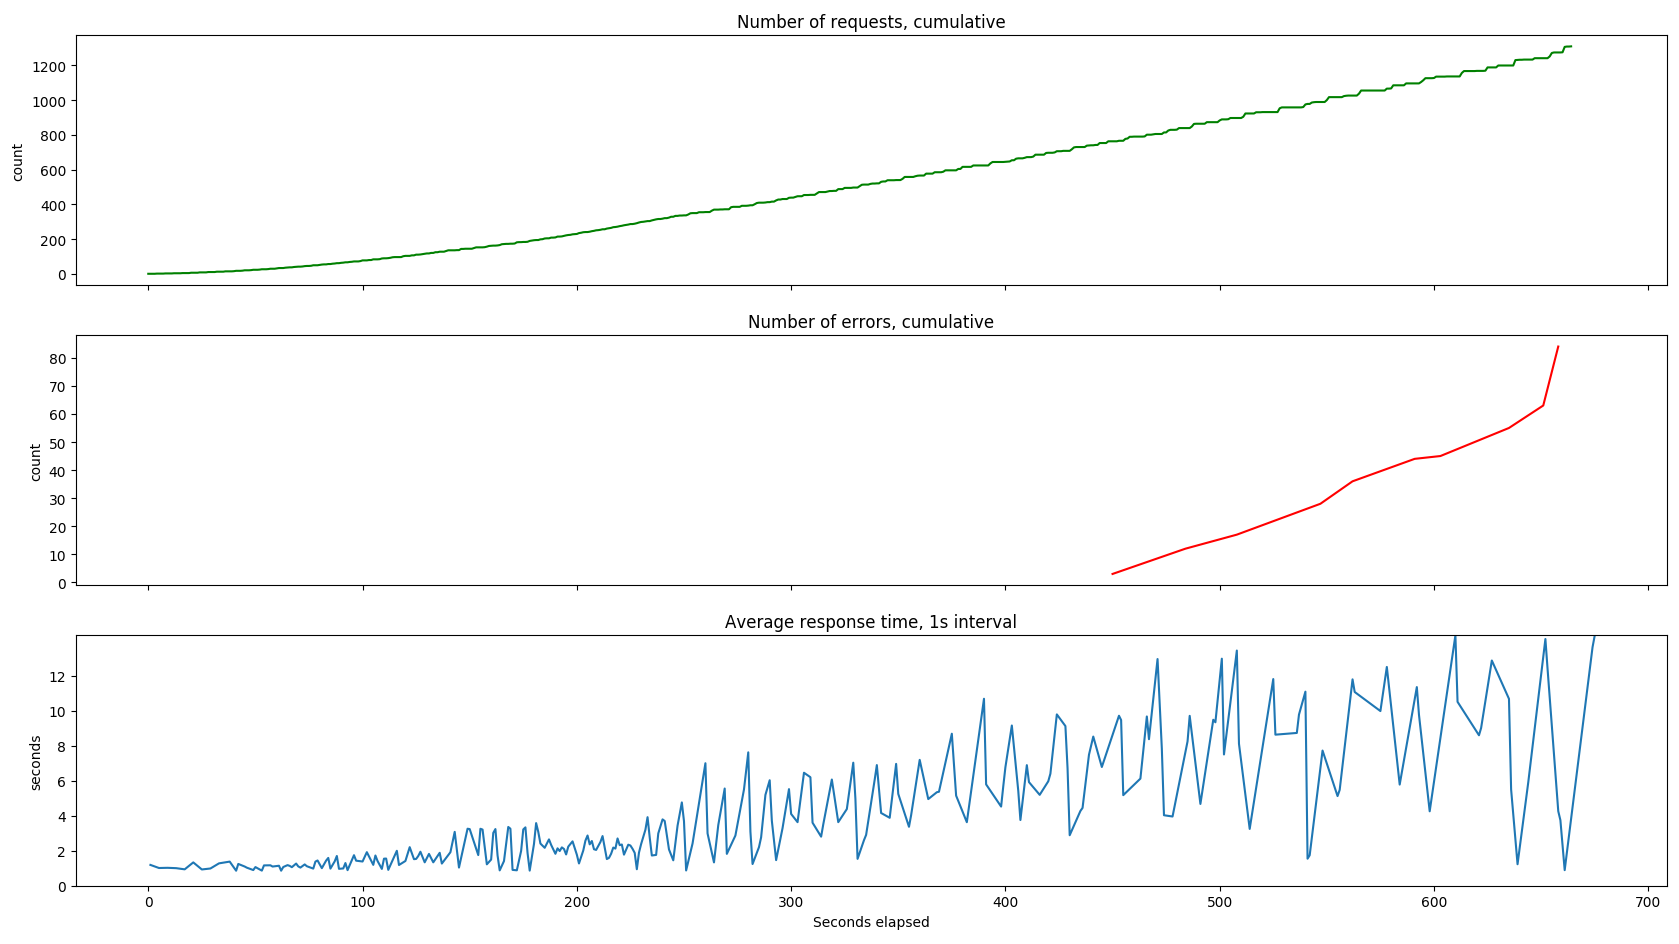
\includegraphics[width=0.9\textwidth]{serverful-load-test.png}
  \caption{Serverful Image Manager load test results}
  \label{fig:serverfulLoadTest}
\end{figure}

\begin{figure}
  \centering
  \begin{subfigure}[b]{0.9\textwidth}
      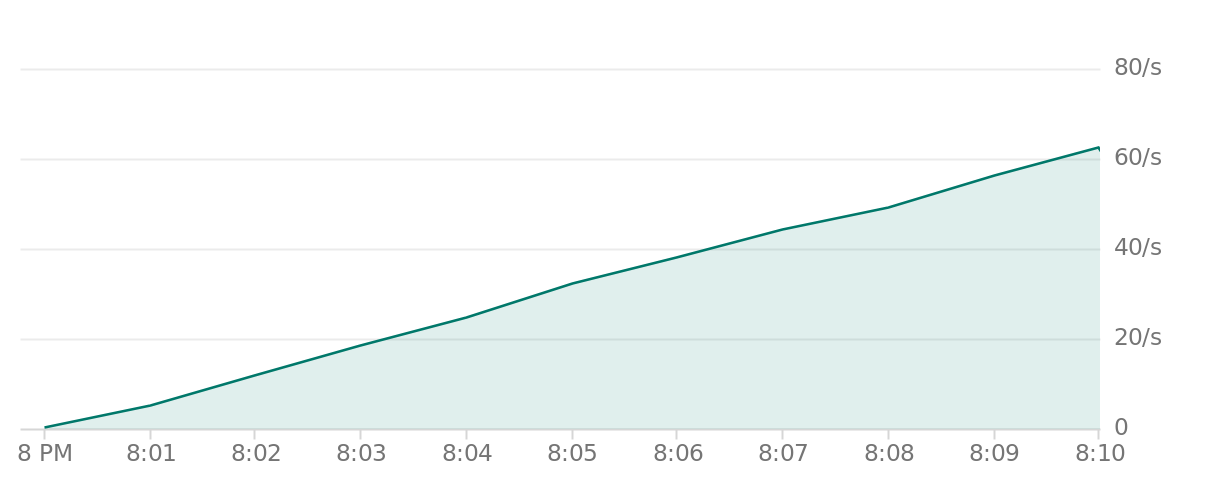
\includegraphics[width=\textwidth]{cloud-functions-invocations-per-second.png}
      \caption{Invocations per second, sum of all functions}
      \label{fig:tiger}
  \end{subfigure}

  \begin{subfigure}[b]{0.9\textwidth}
      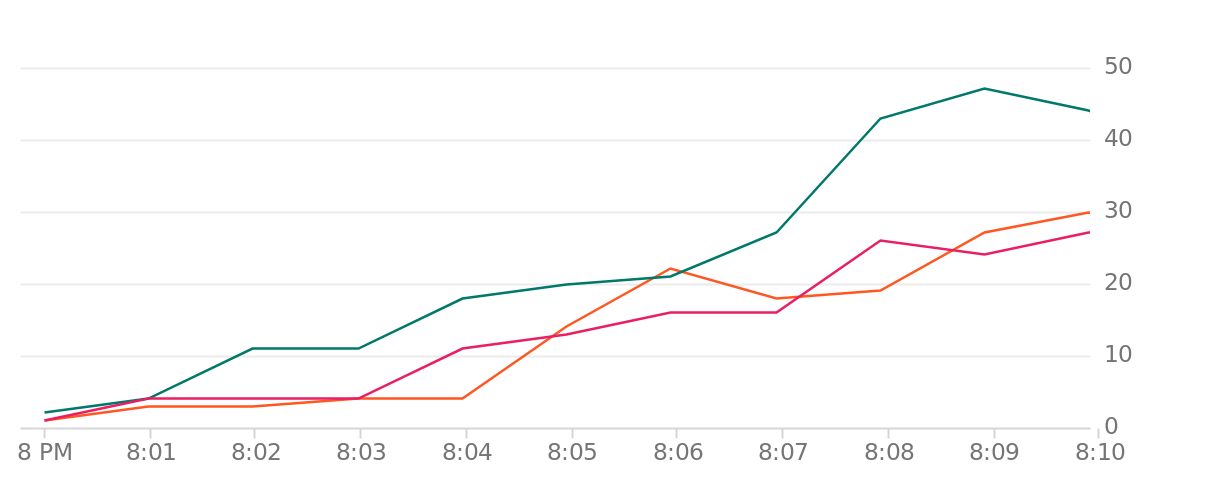
\includegraphics[width=\textwidth]{cloud-function-active-instances.png}
      \caption{Active instances per function}
      \label{fig:gull}
  \end{subfigure}

  \begin{subfigure}[b]{0.9\textwidth}
      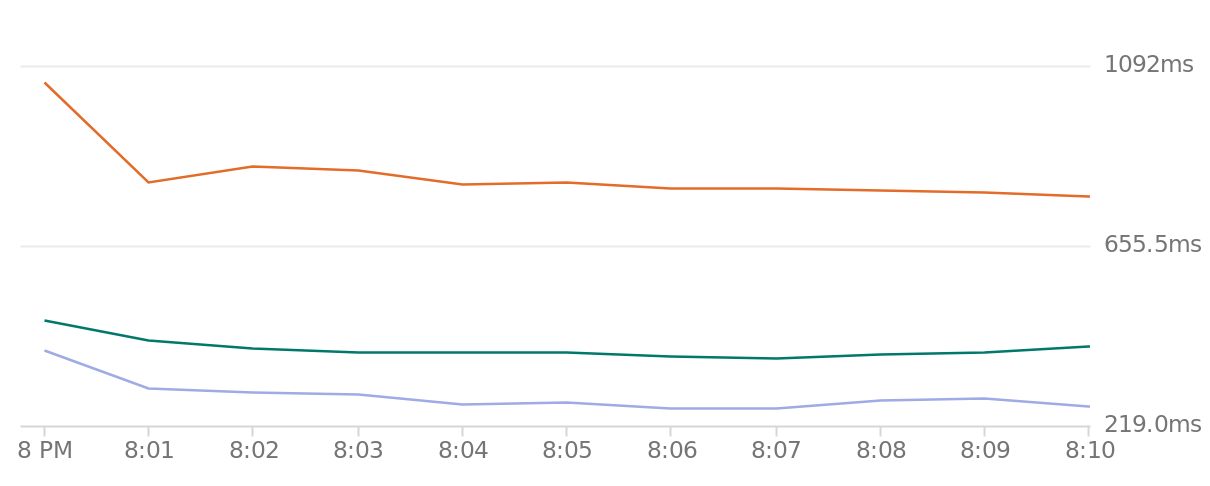
\includegraphics[width=\textwidth]{cloud-function-execution-times-mean.png}
      \caption{Mean execution times per function}
      \label{fig:mouse}
  \end{subfigure}
  \caption{Serverless Image Manager load test results}\label{fig:serverlessLoadTest}
\end{figure}

